\documentclass{standalone}
\usepackage{tikz}
\usepackage{circuitikz}
\usetikzlibrary{positioning}

\begin{document}
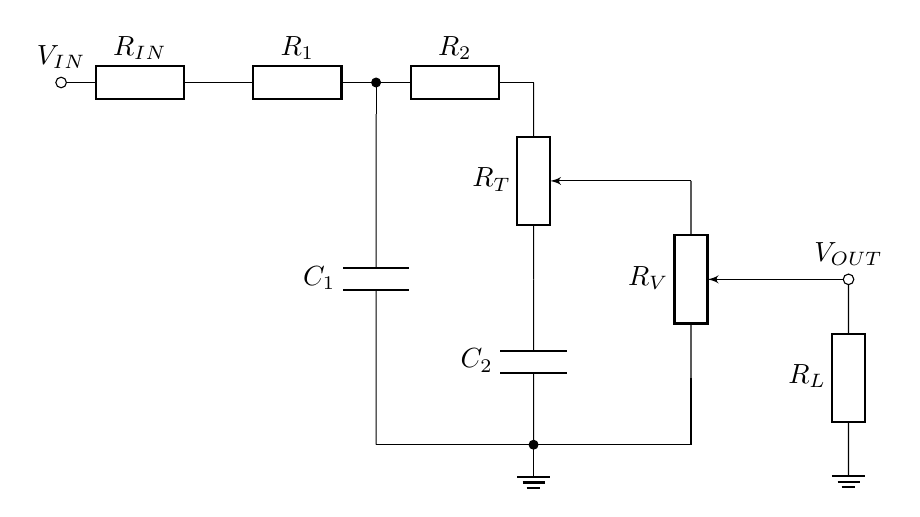
\begin{tikzpicture}
	\draw (-1, 6) to[european resistor, l=$R_{IN}$] (1, 6);	
	\draw (1, 6) to[european resistor, l=$R_1$] (3, 6);
	\draw (3, 6) to[european resistor, l=$R_2$] (5, 6);
	\draw (9, 3.5) to[european resistor, l_=$R_L$] (9, 1);

	\draw (3, 1.4) to[capacitor, l=$C_1$] (3, 5.6);
	\draw (5, 1.4) to[capacitor, l=$C_2$] (5, 3.5);

	\draw (5, 6) to[european potentiometer, l_=$R_T$] (5, 3.5);	
	\draw (7, 4.75) to[european potentiometer, l_=$R_V$] (7, 2.25);

	\draw (3, 5.6) -- (3, 6);
	\draw (5.4, 4.75) -- (7, 4.75);
	\draw (7, 2.25) -- (7, 1.4);
	\draw (9, 3.5) -- (7.5, 3.5);
	\draw (3, 1.4) -- (7, 1.4);	

	\node[ground] at (5, 1.41) {};
	\node[tlground] at (9, 1) {};
	\node[circ] at (3, 6) {};	
	\node[circ] at (5, 1.4) {};	
	\node[ocirc, scale=1.2] at (-1, 6) {};
	\node[ocirc, scale=1.2] at (9, 3.5) {};

	\node[above=0.05cm of {-1, 6}] {$V_{IN}$};
	\node[above=0.05cm of {9, 3.5}] {$V_{OUT}$};

\end{tikzpicture}
\end{document}